% There are two copyright options: copyright and copyright. Seriously,
% the choice boils down to whether you're going to file copyright through
% ProQuest. If you will, use the copyright option.
%\documentclass[dissertation,copyright,notoc,openany]{tufte-book}
\documentclass[dissertation,CC-BY-ND,notoc,openany]{tufte-book}

\setcounter{secnumdepth}{1}
%\setcounter{chapter}{5}

\bibliographystyle{uabibnat}

%%
% To use accents
\usepackage[utf8]{inputenc}

%%
% For nicely typeset tabular material
\usepackage{booktabs}

%%
% For graphics / images
\usepackage{graphicx}
\setkeys{Gin}{width=\linewidth,totalheight=\textheight,keepaspectratio}
\graphicspath{{figs/}}

\usepackage[export]{adjustbox}

% The fancyvrb package lets us customize the formatting of verbatim
% environments.  We use a slightly smaller font.
\usepackage{fancyvrb}
\fvset{fontsize=\normalsize}

%%
% Prints a trailing space in a smart way.
\usepackage{xspace}

%%
% specifying and applying colors
\usepackage{color}

%%
% For table color backgrounds
\usepackage{colortbl}

%%
% for code listings (e.g., R)
\usepackage{listings}

%% color definitions
\definecolor{lightgray}{rgb}{0.96, 0.955, 0.945}
\definecolor{numbergray}{rgb}{0.7, 0.7, 0.7}
\definecolor{midgray}{rgb}{0.5, 0.5, 0.5}
\definecolor{deepred}{rgb}{0.9,0.1,0.1}
\definecolor{lightred}{rgb}{0.975, 0.925, 0.925}

% listing add'l keywords
\lstset{emph={%  
    auc
    },emphstyle={\color{red}}%
}%

\lstdefinestyle{rstyle}{
	language=R,
    backgroundcolor=\color{lightgray},
    commentstyle=\color{midgray},
    keywordstyle=\color{red},
    basicstyle=\scriptsize\ttfamily,
    breakatwhitespace=true,
    breaklines=true,
    keepspaces=true,
    framextopmargin=0pt,
    showspaces=false,
    showstringspaces=false,
    showtabs=false,
    stringstyle=\ttfamily,
    tabsize=2
}
 
\lstset{style=rstyle}

%%
% Sometimes you want a full-page figure with no margin notes.
\newenvironment{pagefigure}{%
	\begin{figure*}[p]
	\classiccaptionstyle
}{\end{figure*}}

%%
% Sometimes you want a full-page table with no margin notes.
\newenvironment{pagetable}{%
	\begin{table*}[p]
	\classiccaptionstyle
}{\end{table*}}

%%
% Would otherwise be `Bibliography', but UA requires `References'
\renewcommand{\bibname}{References}

%%
% Prints argument within hanging parentheses (i.e., parentheses that take
% up no horizontal space).  Useful in tabular environments.
\newcommand{\hangp}[1]{\makebox[0pt][r]{(}#1\makebox[0pt][l]{)}}

%%
% Prints an asterisk that takes up no horizontal space.
% Useful in tabular environments.
\newcommand{\hangstar}{\makebox[0pt][l]{*}}

%%
% Emphasize table result
\newcommand{\redem}[1]{\textcolor{deepred}{\textbf{#1}}}

%%
% mark TODOs
\newcommand{\todo}[1]{\textcolor{red}{TODO: #1}}

%%
% mark edits
\newcommand{\edit}[1]{\textcolor{blue}{#1}}

%%
% Improve chapter title appearance
\makeatletter
\titleformat{\chapter}%
  [block]% shape
  {\relax\ifthenelse{\NOT\boolean{@tufte@symmetric}}{\begin{fullwidth}}{}}% format applied to label+text
  {\itshape\huge\thechapter\quad}% label
  {0pt}% horizontal separation between label and title body
  {\huge\rmfamily\itshape}% before the title body
  [\ifthenelse{\NOT\boolean{@tufte@symmetric}}{\end{fullwidth}}{}]% after the title body
\makeatother

%%
% More space between figure numbers and titles
\makeatletter
     \renewcommand*\l@figure{\@dottedtocline{1}{1em}{2.2em}}
\makeatother

%%
% more space between table numbers and titles
\makeatletter
     \renewcommand*\l@table{\@dottedtocline{1}{1em}{2em}}
\makeatother

%%
% Repeated values, esp in front material.
\completetitle{My Incredible Dissertation}
\fullname{Dale cooper} % Full name (including middle etc.)
\degreename{Doctor of Philosophy}	% Title of your degree.
\title{My short title}
\author{Coop}

% Generates the index, if you create one. (Does nothing, otherwise.)
\usepackage{makeidx}
\makeindex


% since 1995    
\urldef\pubmedquery\url{https://www.ncbi.nlm.nih.gov/pubmed?term=(%221995%22%5BDate%20-%20Publication%5D%20%3A%20%222017%22%5BDate%20-%20Publication%5D)}

% since 1900
\urldef\pubmedquery\url{https://www.ncbi.nlm.nih.gov/pubmed/?term=%221900%22%5BPDAT%5D%20%3A%20%222017%22%5BPDAT%5D&cmd=DetailsSearch}

\usepackage{multirow}
\usepackage{subfigure}
\usepackage{pbox}
\usepackage{bm}
\usepackage{latexsym}
\usepackage{csquotes}
\usepackage{amsmath}
\usepackage{pdflscape}
\usepackage{fancyref}

% for tikz compatibility
%\noautomath
\usepackage{varwidth}
\usepackage{tikz}
\usetikzlibrary{automata, calc, backgrounds, er, trees, fit, positioning, arrows, chains, shapes.geometric, decorations.pathreplacing, decorations.pathmorphing,shapes, matrix, shapes.symbols}
\usepackage{tikz-qtree}
\usepackage{tikz-dependency}
%\usepackage{gb4e}
\usepackage{enumitem}
%\usepackage{subcaption}
%\usepackage[lined]{algorithm2e}

%\bibliographystyle{plainnat}
% \usepackage[american]{babel}
% \usepackage[
%         backend=biber,
%         style=authoryear,
%         sorting=nyt,
%         natbib=true,
%         doi=true,
%         arxiv=abs,
%         url=true
% ]{biblatex}

% \addbibresource{dissertation.bib}
% \DefineBibliographyStrings{american}{phdthesis = {PhD dissertation}}
% \preto\fullcite{\AtNextCite{\defcounter{maxnames}{99}}}


\usepackage{placeins}

\let\Oldsection\section
\renewcommand{\section}{\FloatBarrier\Oldsection}

\let\Oldsubsection\subsection
\renewcommand{\subsection}{\FloatBarrier\Oldsubsection}

\let\Oldsubsubsection\subsubsection
\renewcommand{\subsubsection}{\FloatBarrier\Oldsubsubsection}


\usepackage[framemethod=TikZ]{mdframed}
\mdfdefinestyle{proceduredesc}{%
    linecolor=black,
    outerlinewidth=0.5pt,
    roundcorner=5pt,
    innertopmargin=\baselineskip,
    innerbottommargin=\baselineskip,
    innerrightmargin=15pt,
    innerleftmargin=15pt,
    backgroundcolor=gray!10!white}


\usepackage{epigraph}
\renewcommand{\epigraphsize}{\small}

\setlength{\epigraphwidth}{1.0\textwidth}

\renewcommand{\textflush}{flushright} \renewcommand{\sourceflush}{flushright}

\let\originalepigraph\epigraph 
\renewcommand\epigraph[2]{\originalepigraph{\textit{#1}}{\textsc{#2}}}

\newcommand{\reach}{Reach}
\newcommand{\odin}{Odin}
\newcommand{\grayrule}{}

% define extractor language
\lstdefinelanguage{yaml}{% alsoletter={@=><&?.*+^,_/|[]},
	morestring=[b]", keywords={true, false, null, name, action, example,
		priority, type, label, unit, pattern}, keywordstyle=\textbf,
	ndkeywords={trigger, ?<trigger>, theme, theme?, ?<theme>, @theme,
		cause, cause?, ?<cause>, @cause, site, site?, @site, product,
		product?, @site, controller, controlled, @controlled,
		?<witness>, @witness,
		?<entity>, @entity, entity, word, lemma, tag,
		?<location>, @location, location,
		?<robber>, @robber, robber,
		@property, property,
		agent, vehicle,
		obstacle,
		title,
		@person, person,
		@num,
		dancer, partner,
		city},
	ndkeywordstyle=\color{arsenic}\bfseries, comment=[l]{\#},
	commentstyle=\color{coolgrey}\textit, stringstyle=\ttfamily,
	sensitive=true }

\lstdefinestyle{yaml-style}{%
	language=yaml,
	basicstyle=\ttfamily\footnotesize,
	%basewidth={0.5em,0.5em},
	xleftmargin=9pt,
	xrightmargin=-8pt,
	%xleftmargin=20pt,
	%xrightmargin=-8pt,
	framexleftmargin=16pt,
	framexrightmargin=-10pt,
	%framextopmargin=2pt,
	%framexbottommargin=0pt,
	%frame=trBL,
	%frameround=fttt,
	frame=tb,
	captionpos=t,
	backgroundcolor=\color{anti-flashwhite},
	rulecolor=\color{black},
	extendedchars=true,
	showstringspaces=false,
	showspaces=false,
	numbers=left,
	numberstyle=\tiny,
	numbersep=8pt,
	stepnumber=1,
	tabsize=2,
	breaklines=true,
	showtabs=false,
	escapeinside={(*@}{@*)}
}

\lstnewenvironment{yaml}[1]{%
	\lstset{style=yaml-style}}{%
	\captionof{lstlisting}{#1}
}

%\renewcommand{\lstlistingname}{Rule}% Listing -> Example
\renewcommand{\lstlistingname}{\bfseries Rule}
\makeatletter
\def\fnum@lstlisting{%
  \lstlistingname
  \ifx\lst@@caption\@empty\else~\thelstlisting\normalfont\fi}%
\makeatother

%%%%%%%%%%%%%%%%%%%%%%%%%%%
% custom figures
%%%%%%%%%%%%%%%%%%%%%%%%%%%
\usepackage{float}
\newfloat{example}{thp}{lop}
\floatname{example}{Example}

%%%%%%%%%%%%%%%%%%%%%%%%%%%%
% define colors
\definecolor{lightgray}{gray}{0.7}
\definecolor{anti-flashwhite}{rgb}{0.95, 0.95, 0.96}
\definecolor{coolgrey}{rgb}{0.55, 0.57, 0.67}
\definecolor{arsenic}{rgb}{0.23, 0.27, 0.29}
\definecolor{purpleish}{cmyk}{0.75,0.75,0,0}
\definecolor{light-gray}{gray}{0.9}
\definecolor{light-red}{rgb}{1,.8,.8}
\definecolor{pinegreen}{rgb}{0.0, 0.47, 0.44}
%%%%%%%%%%%%%%%%%%%%%%%%%%%%

\DeclareMathOperator*{\argmin}{argmin}
\DeclareMathOperator*{\argmax}{argmax}

%\newcommand{\todo}[1]{\textcolor{red}{TODO: #1}}
\newcolumntype{x}[1]{>{\centering\arraybackslash\hspace{0pt}}p{#1}}
\definecolor{tbl}{rgb}{.85,.95,.85}

% Render DOIs as URLs
\renewcommand{\doi}[1]{\href{http://dx.doi.org/#1}{\textsc{doi}: #1}}
 
% fix to avoid weird interaction with Tufte
\usepackage{gb4e}
\noautomath
%\usepackage{linguex}

% Add the following code AFTER the gb4e package has been loaded.
% This will restore the Tufte-LaTeX definition of footnotes (as sidenotes)
% but adds in the two lines of code used by the gb4e package.
\makeatletter
\renewcommand\@footnotetext[2][0pt]{%
  \@noftnotefalse\setcounter{fnx}{0}% added by gb4e
  \marginpar{%
    \hbox{}\vspace*{#1}%
    \def\baselinestretch {\setspace@singlespace}%
    \reset@font\footnotesize%
    \@tufte@margin@par% use parindent and parskip settings for marginal text
    \vspace*{-1\baselineskip}\noindent%
    \protected@edef\@currentlabel{%
       \csname p@footnote\endcsname\@thefnmark%
    }%
    \color@begingroup%
       \@makefntext{%
         \ignorespaces#2%
       }%
    \color@endgroup%
  }%
  \@noftnotetrue% added by g4be
}%
\makeatother
% End of Tufte-LaTeX-related code.

\begin{document}

\begin{fullwidth}
% Set up the title page
\maketitlepage
{DEPARTMENT OF LINGUISTICS}	% Title of your department.
{20??}

% Insert the approval form.  Note that for electronic submission
% of your PhD. dissertation, you must bring *two* copies of the
% approval page to your final defense.  These must be signed by
% the committee. 
\approval
{July ??, 20??}		% Defense Date	
{???}		% Co-Chair
{???}    % Co-Chair
{???}	% committee member
{} % 4th committee member (leave empty if None)
{} % 5th committee member (leave empty if None)

% Include the ``Statement by Author'' for Dissertations
\statementbyauthor % Yes, you need the second one of these.
% If this is a Thesis, use the following form, with your thesis director's
% name and title in the square brackets like so (you should also omit the 
% approval form insertion above):
%\statementbyauthor[Jane M. Doe\\Professor of Chemistry]

% Include the ``Acknowledgements''
% NB: Strongly encouraged
\incacknowledgements{acknowledgments}

% Include the ``Dedication''
% NB: optional
\incdedication{dedication}

% Create a ``Table of Contents''
% NB: required
\tableofcontents

% Create a ``List of Figures''
% NB: Strongly encouraged
\listoffigures

% Create a ``List of Tables''
% NB: Strongly encouraged
\listoftables

% Include the ``Abstract''
% NB: required
\incabstract{abstract}

\end{fullwidth}

% Include the various chapters
\chapter{Introduction}
\label{chapter:introduction}
\epigraph{So many books, so little time.}{Frank Zappa}

The aim of this work is to ???.

\section{???}
\label{sec:intro-1}
Since at least 1990, there has been exponential growth in the number of academic papers published annually in the biomedical domain~\citep{pautasso2012publication}.  
The number of English language biomedical citations indexed by PubMed\sidenote[][-2cm]{\url{https://www.ncbi.nlm.nih.gov/pubmed}} alone since 1900 have now surpassed 29 million\sidenote[][-1cm]{\url{https://www.ncbi.nlm.nih.gov/pubmed?term=(\%221990\%2F01\%2F01\%22\%5BDate\%20-\%20Publication\%5D\%20\%3A\%20\%223000\%22\%5BDate\%20-\%20Publication\%5D)}}.

\begin{figure}
  \centering
  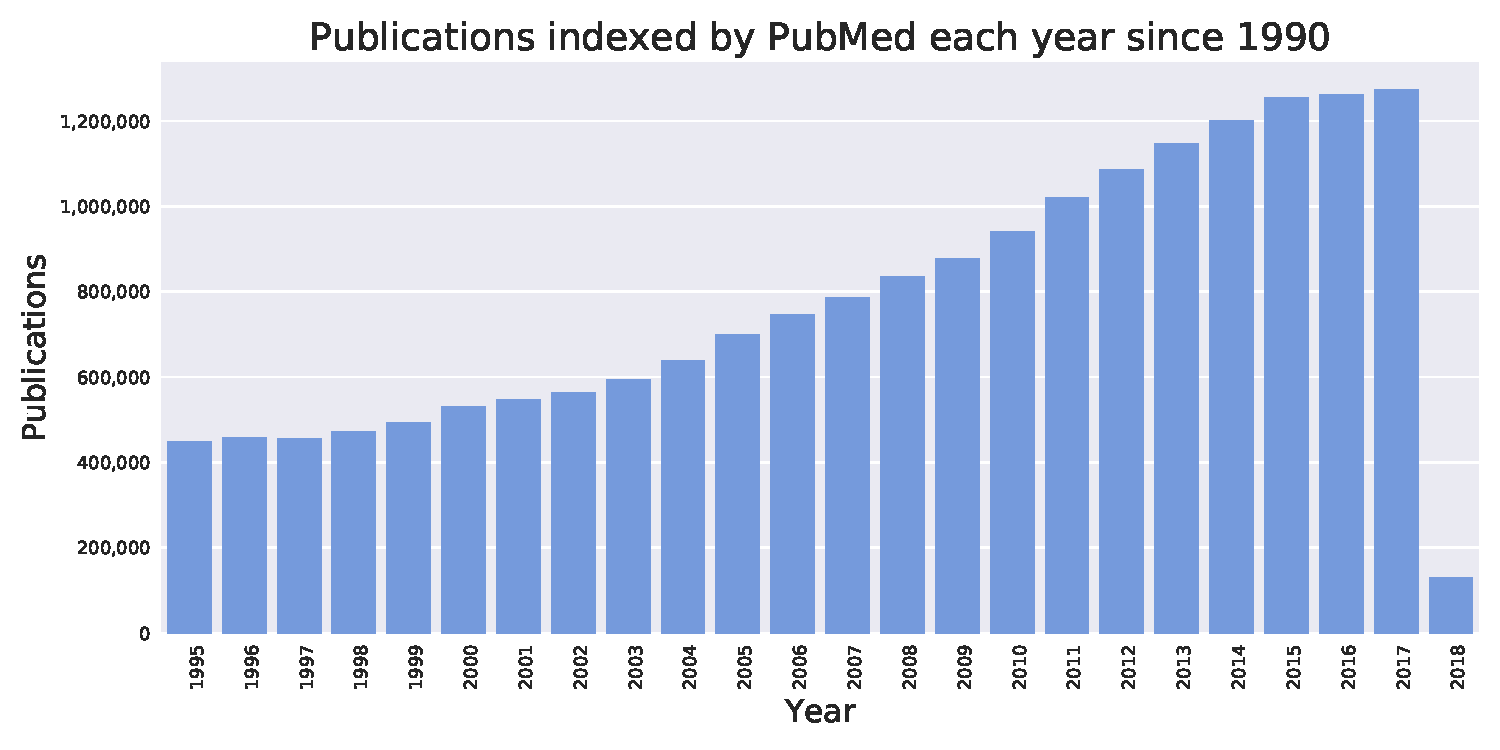
\includegraphics[width=\linewidth]{introduction/pubmed_pub_rate.pdf}
  \caption[][3cm]{According to data indexed by PubMed, biomedical publications remained fewer than 100,000 per year until 1951.  The annual rate began to exceed 1,000,000 in 2011.}
  \label{fig:intro-pubmed-pubs}
\end{figure}

Publications in the domain now exceed 1 million documents per year.  
This poses a serious challenge to researchers needing to understand the state of the field.  
It is effectively impossible for an individual to summarize the larger body of work or even remain abreast of research findings directly relevant to a subtopic.  %\sidenote{Though the severity of the problem has worsened, ~\citet{swanson:1986,swanson1986undiscovered} had already drawn attention to this issue in the 1980s.    
Moreover, how do all of these experimental results interact, and what broader biological context do they define?  
What contradictions exist within the literature?

\chapter{Example}
\label{chapter:example}

\epigraph{There is no magic. There is only knowledge, more or less hidden.}{\textit{Gene Wolfe \\ Shadow \& Claw}}

%\epigraph{You can't connect the dots looking forward; you can only connect them looking backwards.}{Steve Jobs}

\section{Overview}
\label{sec:example-overview}
%\item Explores two types of models for scientific discovery
This chapter examines ??? based on the work introduced in earlier chapters. 
I will begin by outlining a method for ??? in \citet{???}.  
The approach is built upon ??? described in Chapter~\ref{chapter:introduction}.  
%The second model describes how a citation network can be used to derive representations of research communities, which can be used to analyze and rank paths of influence relations.
%We can surface opportunities for collaboration and discovery by identifying disconnected research communities




\section{Conclusions and limitations}
\label{sec:example-conclusion}
\paragraph{Innovation 1} In this chapter I have described how ???.  
While our initial results are modest, the ???.  Results would likely improve by ???, as well as exploring ???.

\chapter{Conclusions}
\label{chapter:conclusion}

\section{Summary}
In this work, I have argued that ???.

% Include the various appendices
%\backmatter
\appendix
%\include{chapters/odin-appendix}
\include{chapters/example-appendix}

\backmatter
\begin{fullwidth}
%%
% Formatting notes
% Remember that the Grad College insists their be no blank pages.
% I use pdftk for this, e.g.,
% pdftk A=dissertation.pdf B=watermarked_signatures.pdf cat A1 B1 3-end output dissertation_signed.pdf
% pdftk A=dissertation.pdf B=watermarked_signatures.pdf cat A1 B1 3-91 93-end output dissertation_signed.pdf
% The above command takes the output of this file, substitutes a water-
% marked signature page for the second page, then cuts out page 92, and
% saves the result in dissertation_signed.pdf.
%\clearpage
%\setcounter{page}{114}
\let\clearpage\relax
% Create the References list
\bibliography{dissertation}
\end{fullwidth}

\end{document}
